\documentclass[12pt,a4paper]{amsart}
%\usepackage[slovene]{babel}
\usepackage[utf8]{inputenc}
%\usepackage[T1]{fontenc}
\usepackage{amsmath,amssymb,amsfonts}
\usepackage[dvipsnames,usenames]{color}
\usepackage{algorithmicx,algpseudocode}
\usepackage{graphicx}

\textwidth 15cm
\textheight 24cm
\oddsidemargin.5cm
\evensidemargin.5cm
\topmargin-5mm
\addtolength{\footskip}{10pt}
\pagestyle{plain}

\overfullrule=15pt % oznaci predlogo vrstico

\newtheorem{definition}{Definition}[section]
\newtheorem{lemma}[definition]{Lemma}
\newtheorem{theorem}[definition]{Theorem}
\newtheorem{corollary}[definition]{Corollary}

\def\R{\mathbb R}
\def\N{\mathbb N}
\def\Z{\mathbb Z}
\def\C{\mathbb C}
\def\Q{\mathbb Q}

\begin{document}

\thispagestyle{empty}
\noindent{\large
University of Ljubljana \hfill  \today\\[1mm]
Faculty of Computer and Information Science  \\[5mm]
%IŠRM -- 2.~stopnja
}
%\vfill
\begin{center}{\large
Computational topology\\[4mm]
% Seminarska naloga\\[4mm]
{\bf Text classification using persistent homology}\\[4mm]
Matija Čufar, Domen Keglevič\\[6mm]
}
\end{center}
\bigskip

\section{Introduction}

\emph{TODO: nekaj o vztrajni homologiji in mogoče analizi teksta}

In this report, we attempt to classify texts from four different domains by
comparing their persistence diagrams.

\section{Methods}

We have chosen to attempt to classify texts from the following domains:

\begin{itemize}
\item Excrepts from the Old and New Testaments of the Bible,
\item abstracts of articles from phys.org,
\item recipes from allrecipes.com.
\end{itemize}

For each of the domains, we picked ten texts, each at least 100 words long. We
used the Gudhi library~\cite{maria2014gudhi} to compute persistent homology on
the texts.

We used the following two approaches to build simplicial complexes for each of
the domains:

\subsection{Feature-based Alpha and Vietoris-Rips complexes}

Our first approach involved computing the following features for each of the
texts:

\begin{itemize}
  \item the ratio of (average word length)/(longest word length),
  \item the ratio of (average sentence length)/(longest sentence length),
  \item the ratio of the total number of three words with the highest tf-idf
    value among all the words,
  \item the ratio of the number of words of length $\le 8$ among all words,
  \item the ratio of the number of words of length $\ge 9$ among all words.
\end{itemize}

This gives us a point in five-dimensional space for each of the texts. We used
these points to build Alpha and Vietoris-Rips complexes on each of the domains.

\subsection{Distribtuion distance-based Vietoris-Rips complexes}

Our second approach involved computing the distributions of word and sentence
lengths and calculating the distances between the texts using the following
distance measures:

\begin{itemize}
\item The Hellinger distance:

\begin{equation*}
  H(P,Q) = \sqrt{\frac{1}{2} \sum_{i=1}^k\left(\sqrt{p_i} -
    \sqrt{q_i}\right)^2}\ ,
\end{equation*}

\item the Chi-squared distance:

\begin{equation*}
  \chi^2(P,Q) = \frac{1}{2} \frac{(p_i - q_i)^2}{p_i + q_i + \varepsilon}\ ,
\end{equation*}

\item the Euclidean distance:

\begin{equation*}
  E(P,Q) = \sqrt{\sum_{i=1}^k\left(p_i - q_i\right)^2}\ ,
\end{equation*}
\end{itemize}

\noindent
where $P$ and $Q$ are the discrete distributions and $p_i$ and $q_i$ are the
$i$-th bins of those distributions. The $\varepsilon$ in the Chi-squared
distance is a small constant used to avoid dividing by zero.

We used these distances to compute a distance matrix for each of the
domains and used the distance matrices to build Vetoris-Rips complexes.

\subsection{Domain comparsion}

When the simplicial complexes were built, we calculated persistence diagrams for
each complex and computed the bottleneck distances between them.

\section{Results}

% Template za matriko
\begin{table}
  \centering
  \begin{tabular}{l|llll}
                  & Old Testament & New Testament & phys.org & recipes \\ \hline
    Old Testament & 0 & 0 & 0 & 0 \\
    New Testament & 0 & 0 & 0 & 0 \\
    phys.org      & 0 & 0 & 0 & 0 \\
    recipes       & 0 & 0 & 0 & 0 \\
  \end{tabular}
  \caption{The distance matrix}
  \label{tab:}
\end{table}

\begin{figure}
  \centering
  %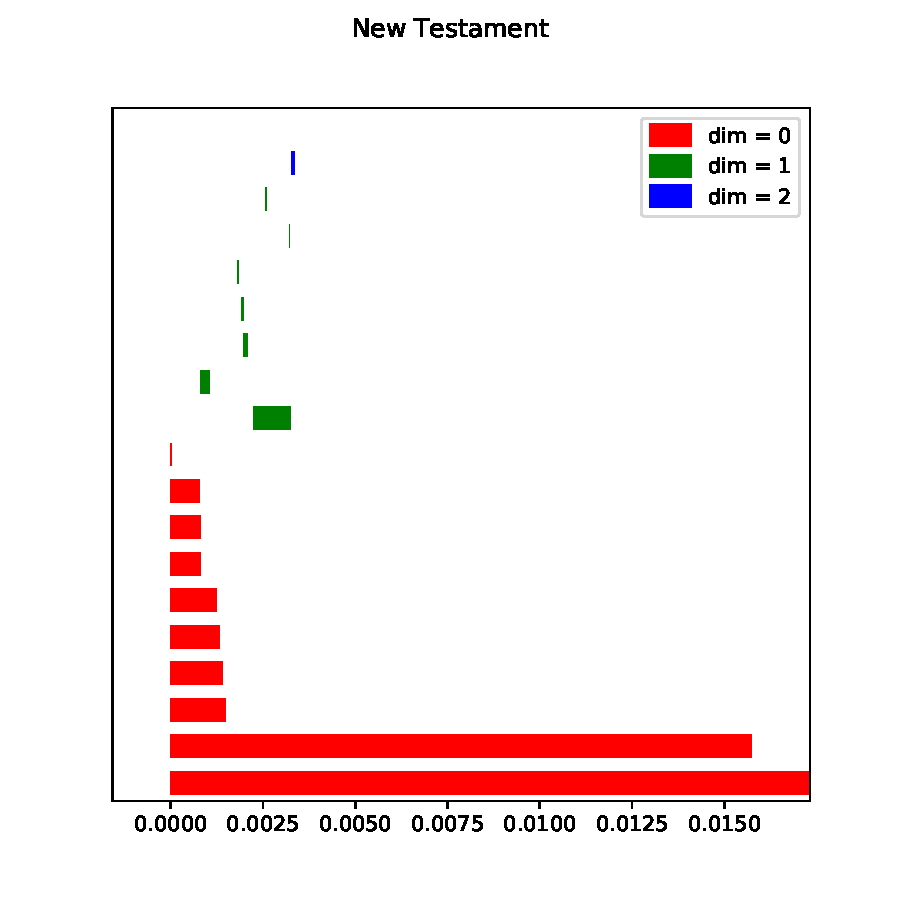
\includegraphics[width=0.4\textwidth]{../plots/barcodes/bible-new}
  %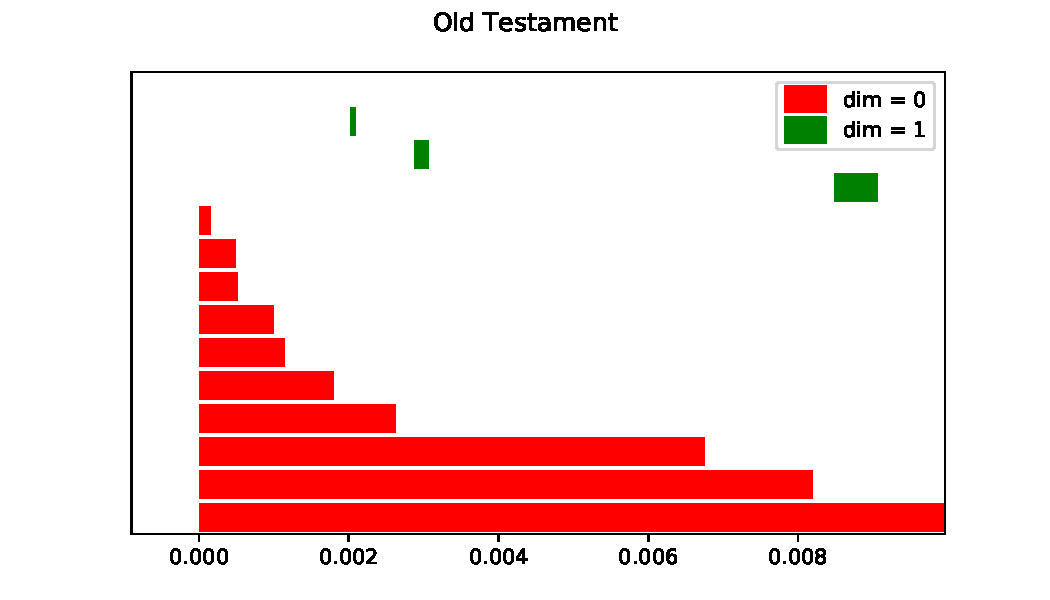
\includegraphics[width=0.4\textwidth]{../plots/barcodes/bible-old}
  %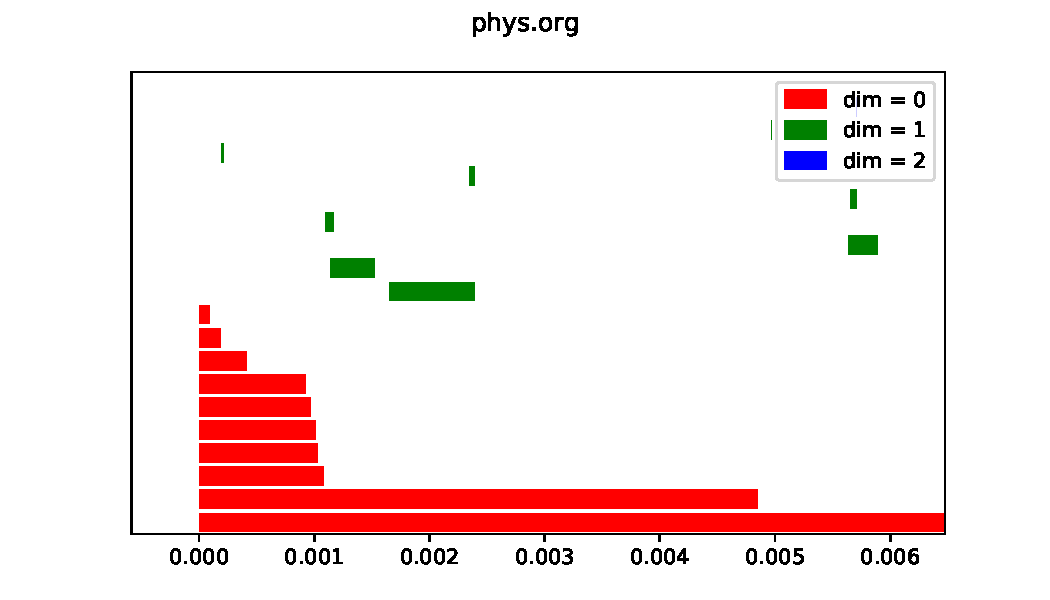
\includegraphics[width=0.4\textwidth]{../plots/barcodes/phys}
  %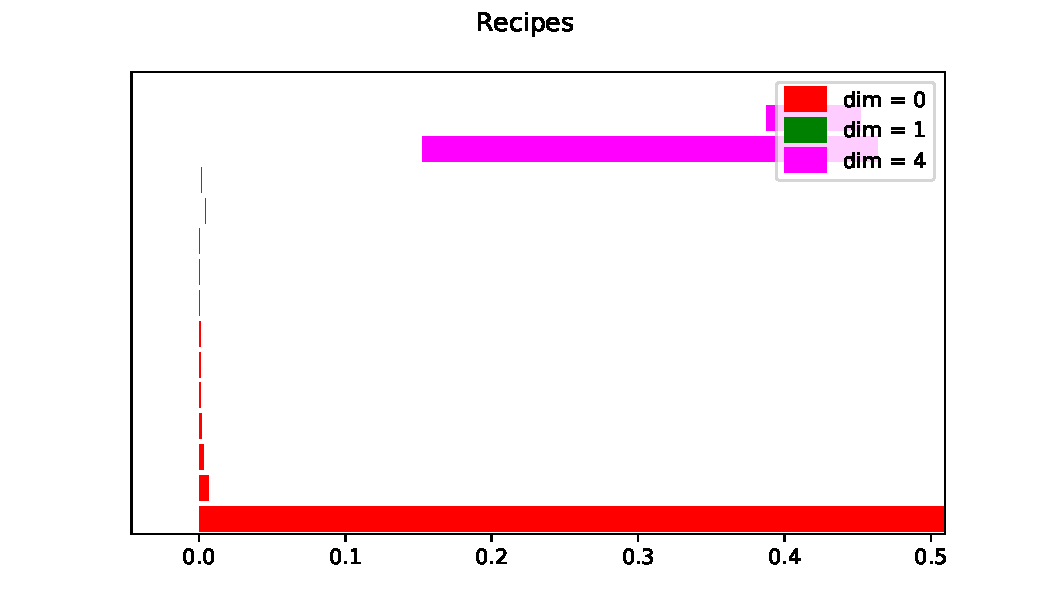
\includegraphics[width=0.4\textwidth]{../plots/barcodes/recipes}
  \caption{TODO: grafi}
  \label{fig:barcode:alpha}
\end{figure}

\section{Conclusion}

\emph{TODO: rezultati so slabi itd}

\emph{TODO: kaj bi blo za probat}

\section{Authors contributions}

% biblio
\bibliographystyle{plain}
\bibliography{biblio}


\end{document}
